\label{sec:empirics}
\subsection{Difference-in-differences panel regression}
The fundamental assumption is that merging of municipalities cause a positive shock to the power of the individual politician as the ratios of population/politicians and expenditure/politician increase. Thus, the firms being treated are those that are connected through family-ties to a politician that at the beginning of a period $t$ is elected in an unmerged municipality and at the end of the period $t+s$ still is elected but now the municipality has merged.

Several measures of profitability could be tried out for the dependent variable $y$, especially operating returns on assets (OROA), sales, and gross profits. All measures could be industry-adjusted as further robustness control.
\\ \\
While the administrative reform in Denmark allowed for difference-in-differences evaluation around the all-at-once implementation \citep{amore2013value}, the continuous merging of municipalities in Japan through more than a decade gives other opportunities. I suggest a time series regression of separate difference-in-differences specifications of length $s$ as shown in equation \ref{eq:FD}. That it, panels of firms are constructed for each period $t\in 1999,\cdots,2010$ with the limit that the firms in any panel for both period $t$ and $t+s$ should have a non-negative book value of assets and have family-ties to an elected politician. The latter is to aspire to comparability of treated and counterfactuals.
\begin{equation}
  \Delta y_{it} = \beta_1\cdot T + \eta\cdot \bm{y}_{i,t-1} + \Delta\gamma_t^c \bm{x}_{i}^c + \gamma^v\cdot\Delta\bm{x}_{it}^v + \Delta u_{it}
  \label{eq:FD}
\end{equation}
To control for heterogeneity in firms a vector of lagged measures of profitability $\bm{y}_{i,t-1}$  could be included or left out. $\bm{x}_i^c$ is the time-invariant characteristics of the firm and municipality for which the effect $\gamma_t^c$ is allowed to change over time. On the contrary, $\Delta \bm{x}_it^v$ is a vector of the differences in time-variant characteristics for the firm and municipality for which the effect $\gamma^v$ is constant over time. Also, time dummies for each year should be included though suppresse in the equation to control for business cycles.

A core extension would be to look at sample split effects for firms in sectors more dependent on contracting with the public sector.

\subsection{Robustness checks}
A potential endogeneity problems from politicians self-selecting into treatment can possibly be solved using a 2SLS approach where instead of a dummy for treatment, it is constructed as a dummy for being a connected firm times a instrument for a merger. That is, \citet{miyazaki2013municipal} has shown that is is feasible to obtain quite precise estimates of the probability of merging.

Similar to \citet{amore2013value} falsification tests and attempts to validate causality should be applied where feasible. First of all testing that trends are similar in the pre-treatment period and also that non-connected firms does not benefit equivalently from merging. A series of sample split results should be conducted as well to look at different effects depending on a) the toughness of electoral competition b) importance of the politician c) size of the firm d) profitability of the firm e) type of municipality.

We are not able to take advantage of a sharp Regression Discontinuity Design, but to ensure that the effect is not biased from mostly comparing rural municipalities with metropolitan municipalities we could try to drop bigger municipalities from the sample or drop all municipalities that are not merged at some point, though the number of contrafactuals will tend to zero if we do not exclude some periods from the estimation. Indeed, the map in figure \ref{fig:prefectures} show that less than 20\% of municipalities are merged in the major metropolitan areas of Tokyo and Osaka as well as in their adjacent prefectures of Yokohama and Nara.
\begin{figure}[H]
  \centering
  \caption{Share of municipalities merged by the 47 prefectures}
    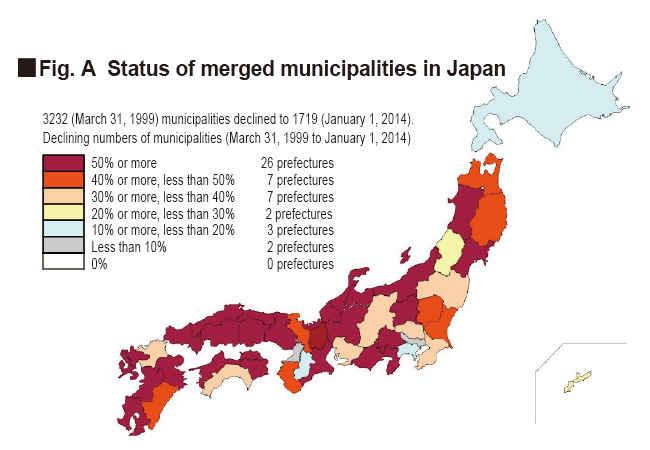
\includegraphics[width= \textwidth]{03_figures/prefectures}
   \sourcec{Ministry of Internal Affairs and Communications.}
  \label{fig:prefectures}
\end{figure}
